\section{Descrição do problema}

\begin{frame}{Variáveis de decisão}
    \begin{itemize}
        \item $x_{ijlkt}$ indica se a bobina $k$ está na posição (i, j) do espaço disponível no momento $t$
\begin{itemize}
    \item $i \in \{1..I\}$ - Índice longitudinal do espaço
    \item $j \in \{1..J\}$ - Índice latitudinal do espaço
    \item $l \in \{0..2\}$ - Índices vertical do espaço
    \item $k \in \{1..K\}$ - Índice das bobinas produzidas
    \item $t \in \{1..T\}$ - Índice dos intervalos para execução de tarefas
\end{itemize}
        \item $m_{kt}$ indica a maquina $m$ move a bobina $k$ na unidade de tempo $t$
        \item $C_{movimento}$ custo de movimento da bobina $k$ no intervalo $t$
    \end{itemize}
\end{frame}

\begin{frame}{Função objetivo}
\begin{itemize}
    \item Desejamos minimizar o custo de movimentar a bobina $k$ no tempo $t$, considerando a prioridade de movimento $p_k$.
    $$min \sum_k\sum_tC_{movimento}(t, k). p_k$$
\end{itemize}
\end{frame}

\begin{frame}{Restrições}
    \begin{block}{1. Cada bobina ocupa exatamente uma posição}
       % $$\sum_{i = 1}^I\sum_{j=1}^J\sum_{k=1}^K\sum_{t=1}^Tx_{ijkt}\leq 1$$
       $$\sum_{i,j}x_{k} = 1$$
        
        $$\forall i,j,k \in \{1..I\},\ j \in \{1..J\},\ k \in \{1..K\}$$
    \end{block}

    \begin{block}{2. Uma maquina só pode mover uma bobina por vez}
        $$\sum_{t = 1}^T\sum_{k=1}^Km_{kt} \leq 1$$
    \end{block}
\end{frame}

\begin{frame}{Restrições}
    \begin{block}{3. O custo de movimentação é calculado proporcionalmente ao movimento do guindaste}
        $$C_{movimento} = (i + j + 2l)\ E\ \forall i,j \in\ \{1..I\},\ \{j..J\}$$
    \end{block}
    \begin{block}{4. Cada bobina tem que ficar parada no armazém por, no mínimo, 3 dias}
        $$\sum_{k} k_{t_{s}}-k_{t_{e}} \geq 72\ \forall\ k \leq K$$
        Onde $k_{t_{e}}$ é o tempo em que a bobina chega no armazém e $k_{t_{s}}$ é o momento de saída.
    \end{block}
\end{frame}

\begin{frame}{Restrições}
    \begin{block}{5. As bobinas podem ser empilhadas respeitando limites de peso}
        $$W_{jkl} \leq W_{jk(l-1)} + W_{j(k + 1)(l - 1 )}$$
        $$ \forall\ k\ k\leq K$$        
        $$ \forall\ l\ \leq 3 $$
        $$ \forall\ j \leq J - l + 1$$
    \end{block}
\end{frame}
\begin{frame}{Restrições}
    \begin{block}{5. As bobinas podem ser empilhadas respeitando limites de peso}
        $$W_{jkl} \leq W_{jk(l-1)} + W_{j(k + 1)(l - 1 )}$$
        $$ \forall\ k\ k\leq K$$        
        $$ \forall\ l\ \leq 2 $$
        $$ \forall\ j \leq J - l$$
    \end{block}
\end{frame}
\begin{frame}{Restrições}
    \centering
         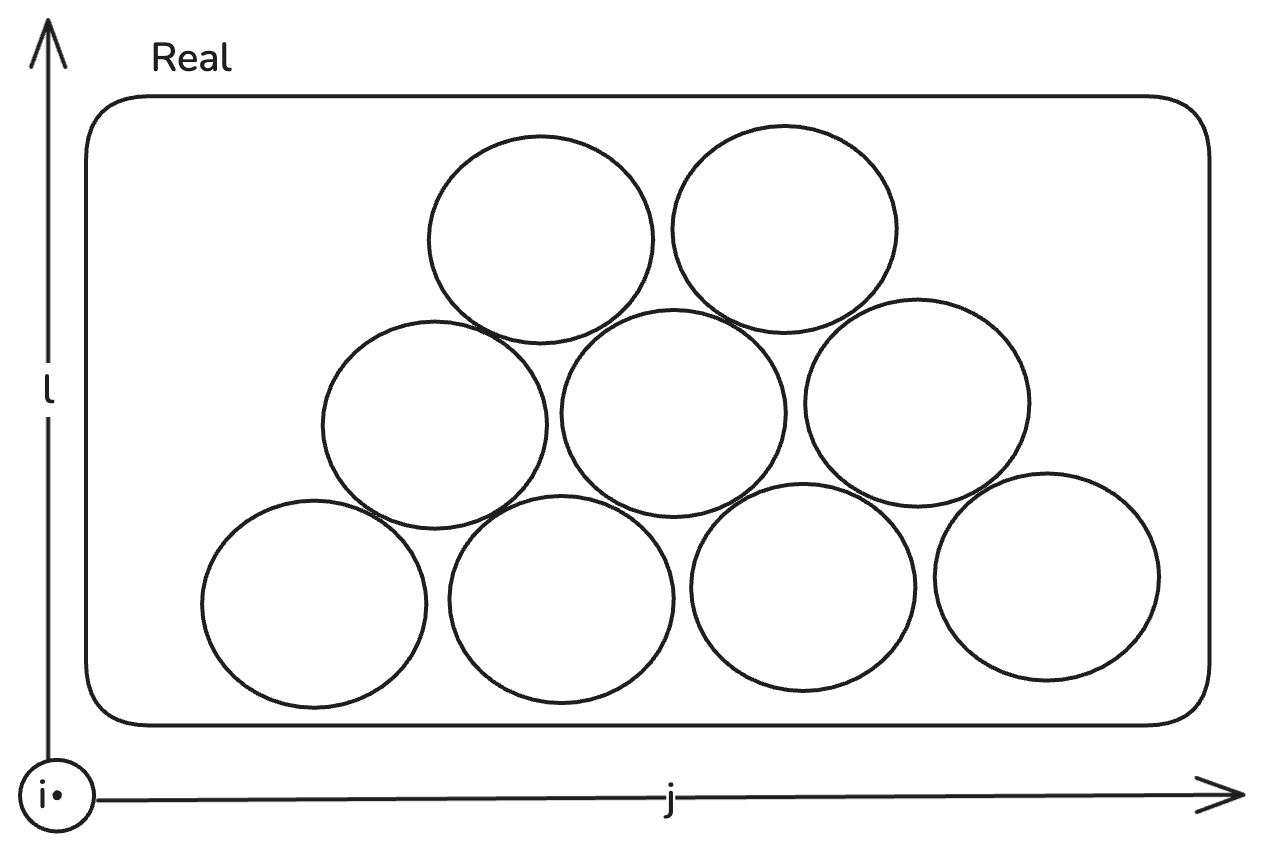
\includegraphics[width=0.55\linewidth]{imagens/modelo-peso-real.png}
\end{frame}
\begin{frame}{Restrições}
    \centering
         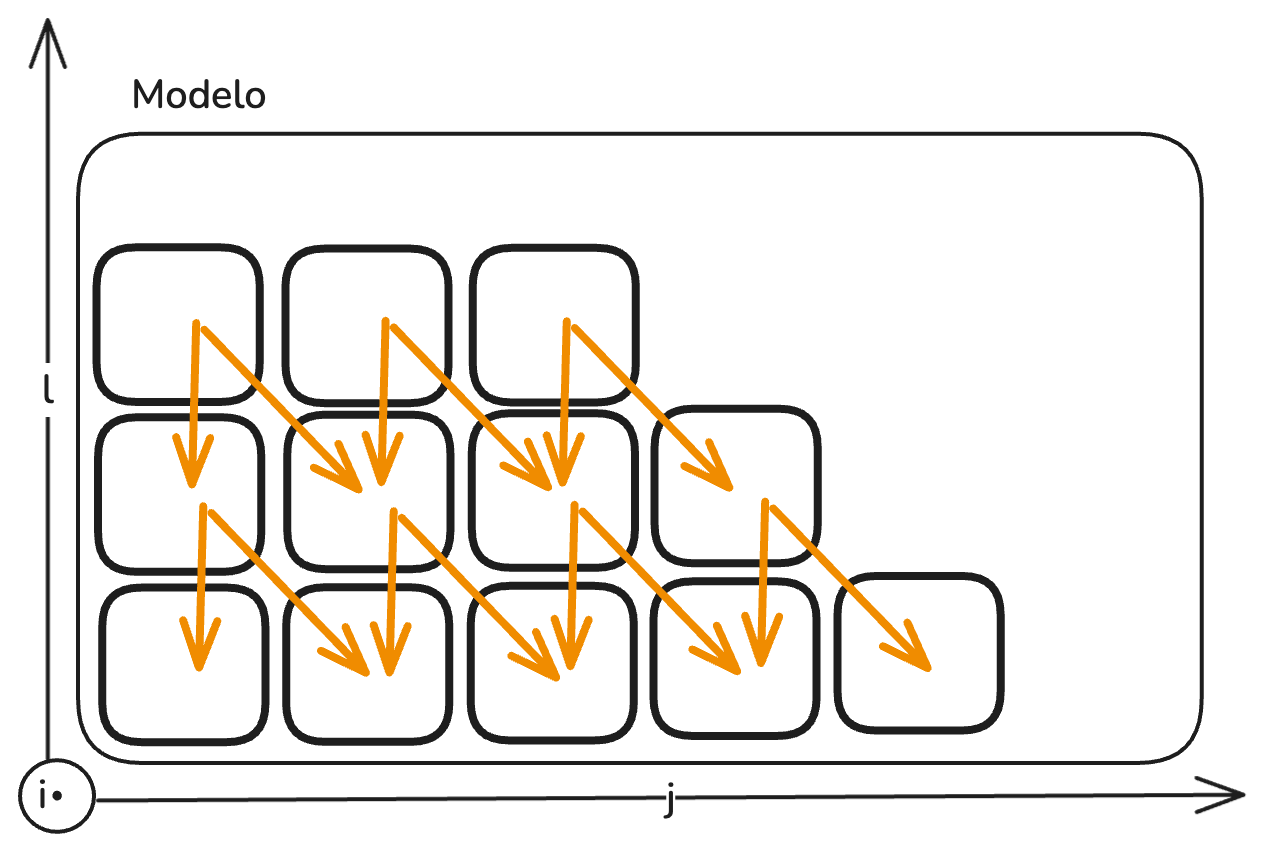
\includegraphics[width=0.55\linewidth]{imagens/modelo-peso-model.png}
\end{frame}
\begin{frame}{Domínio}
    \[
    x_{ijlkt} =
    \begin{cases}
        1, & \text{se a bobina $k$ est\'a na posi\c{c}\~ao $(i, j, l)$ na unidade de tempo $t$} \\
        0, & \text{caso contr\'ario}
    \end{cases}
    \]
\end{frame}
%\begin{frame}{Custo computacional}
% Não precisa ser abordado aqui. Deve ficar para o próximo seminário.   
%\end{frame}

% Ainda não estou muito consciente se posso  fazer uma modelagem por hora
% Se eu modelar hora a hora eu terei que fazer restrições específicas de cada hora 
% isso pode ficar complicado quando temos 24h de operação. 

